\subsubsection{Isotopics}\label{sec:isotopics}
LuRaCs provides a library of data for a selection of common radionuclides that can be accessed under the tab Isotopics. This datacan be used to draw reference lines for emissions in the spectrum plot. Most of the nuclide data is sourced from \textit{Laboratoire National Henri Becquerel}, the others from sources elsewhere. A citation is provided for each nuclide whereas full references can be found under \texttt{Help -> Bibliography}.

\begin{figure}[H]
    \centering
    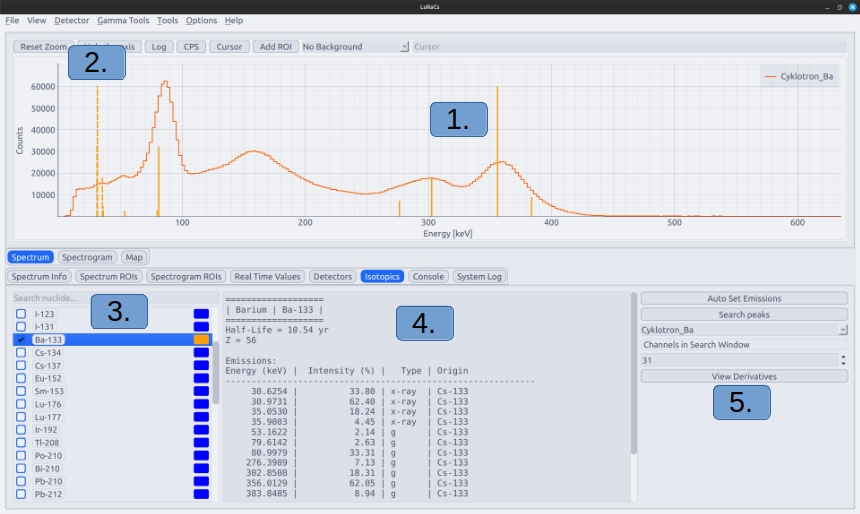
\includegraphics[width = .9\linewidth]{images/interface/isotopics.jpg}
    \caption{Ba-133 spectrum with Ba-133 selected in the Isotopics Tab.}
    \label{fig:isotopics}
    \begin{flushleft}
        \begin{enumerate}
            \item Spectrum and gamma emission lines, drawn as solid lines. Line height corresponds to emission intensity,
            \item X-ray emission lines, drawn as dashed lines. Line height corresponds to emission intensity.
            \item Nuclide list, select nuclide with the checkbox to the left and change colour of the gamma emission lines with the right coloured button.
            \item Information of the current marked nuclide.
            \item Peak automation, see bellow.
        \end{enumerate}
    \end{flushleft}
\end{figure}

Auto matching nuclides to ROIs is accomplished by using the centroid of a fitted peak and finding emission close in energy. The matching is weighted by the emission intensity so a strong emission will be chosen over a weak if they are the same distance from the peak centroid. By selecting nuclides the auto matching of nuclides to ROIs, including from using the button inside the \textit{ROI Editor}, are limited emission from the selected nuclides. Using auto match nuclides against all possible candidates are often unreliable, especially if the energy calibration is imperfect. 

The peak search is based on Savitzky-Golay smoothing and the filter derivatives to compute peak candidates. The computed candidates are filtered, the accepted peaks are then added as ROIs. The length of the window in the Savitzky-Golay filter can be set in units of channels. 